% --- Verzeichnisse ------------------------------------------------------
\newpage
\chapter{Abbildungen}

\begin{figure}[htbp]
    \centering 
		        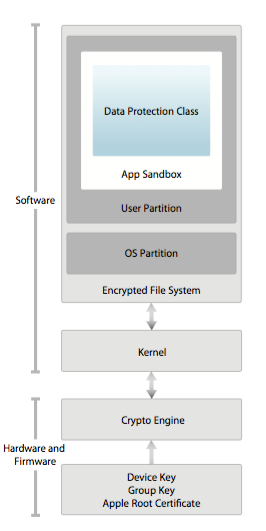
\includegraphics[scale=0.6]{Bilder/SecArchitektur-iOS7.png}
	\caption {iOS Security Architektur iPhone 5c (\cite{Apple[9]} S.3)}
    \label{fig:iOSSecurityArchitekturiOS7}
\end{figure}

\begin{figure}[htbp]
        \centering
                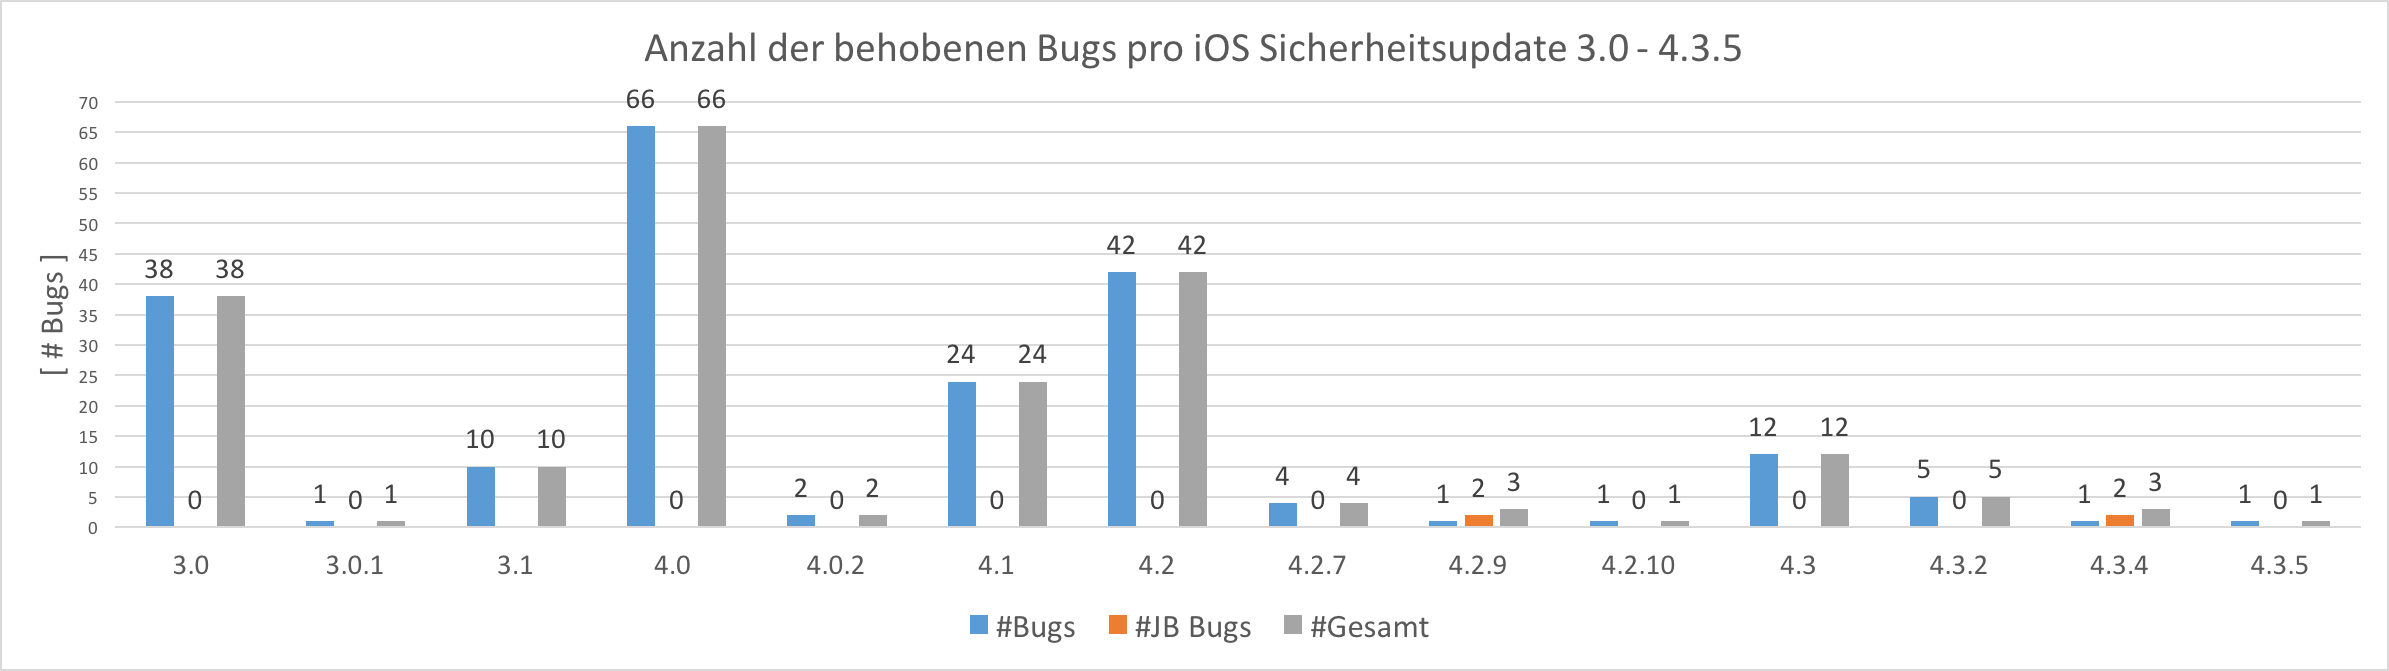
\includegraphics[scale=0.4]{Bilder/iOSSicherheitsupdate3.png}
        \caption{Anzahl Bugs iOS-Sicherheitsupdate iOS Version 3.x - 4.x}
        \label{fig:AnalyseiOSSicherheitsupdate3}
\end{figure}
     
\begin{figure}[htbp]
        \centering
                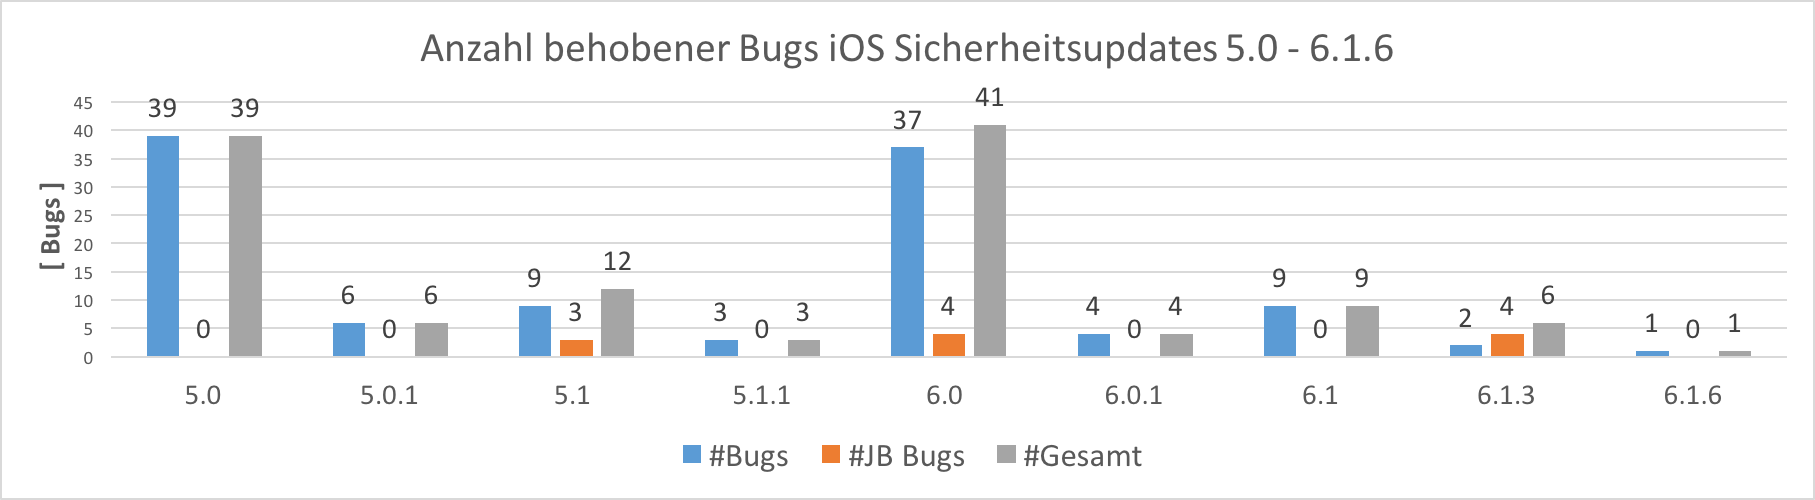
\includegraphics[scale=0.55]{Bilder/iOSSicherheitsupdate5.png}
        \caption{Anzahl Bugs iOS-Sicherheitsupdate iOS Version 5.x - 6.x}
        \label{fig:AnalyseiOSSicherheitsupdate5}
\end{figure}

\begin{figure}[htbp]
        \centering
                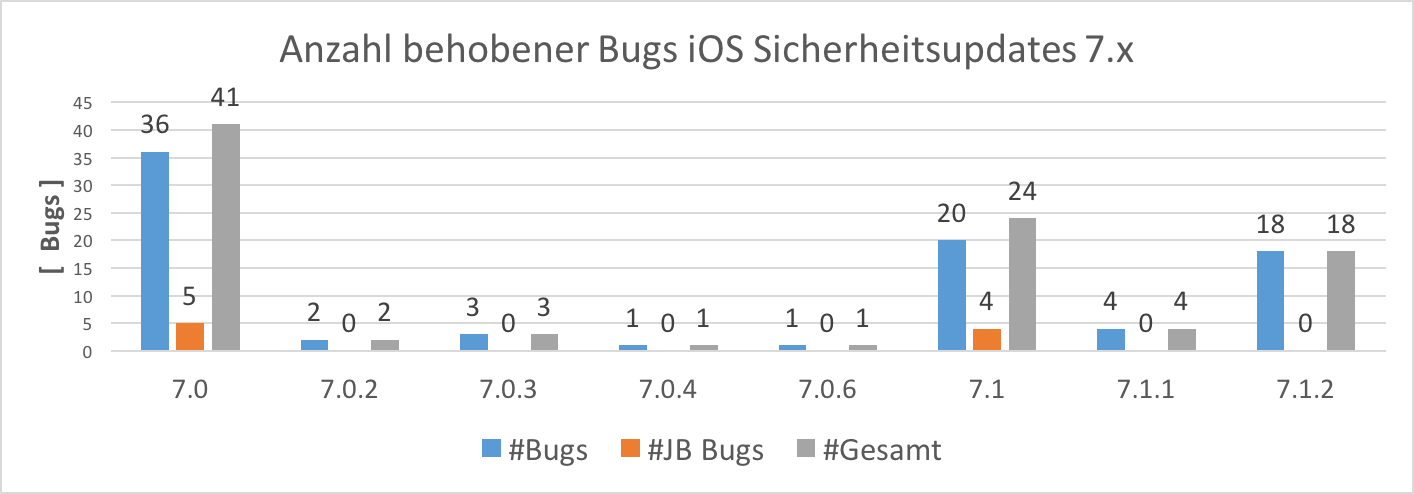
\includegraphics[scale=0.7]{Bilder/iOSSicherheitsupdate7.png}
        \caption{Anzahl Bugs iOS-Sicherheitsupdate iOS Version 7.x}
        \label{fig:AnalyseiOSSicherheitsupdate7}
\end{figure}

\begin{figure}[htbp]
        \centering
                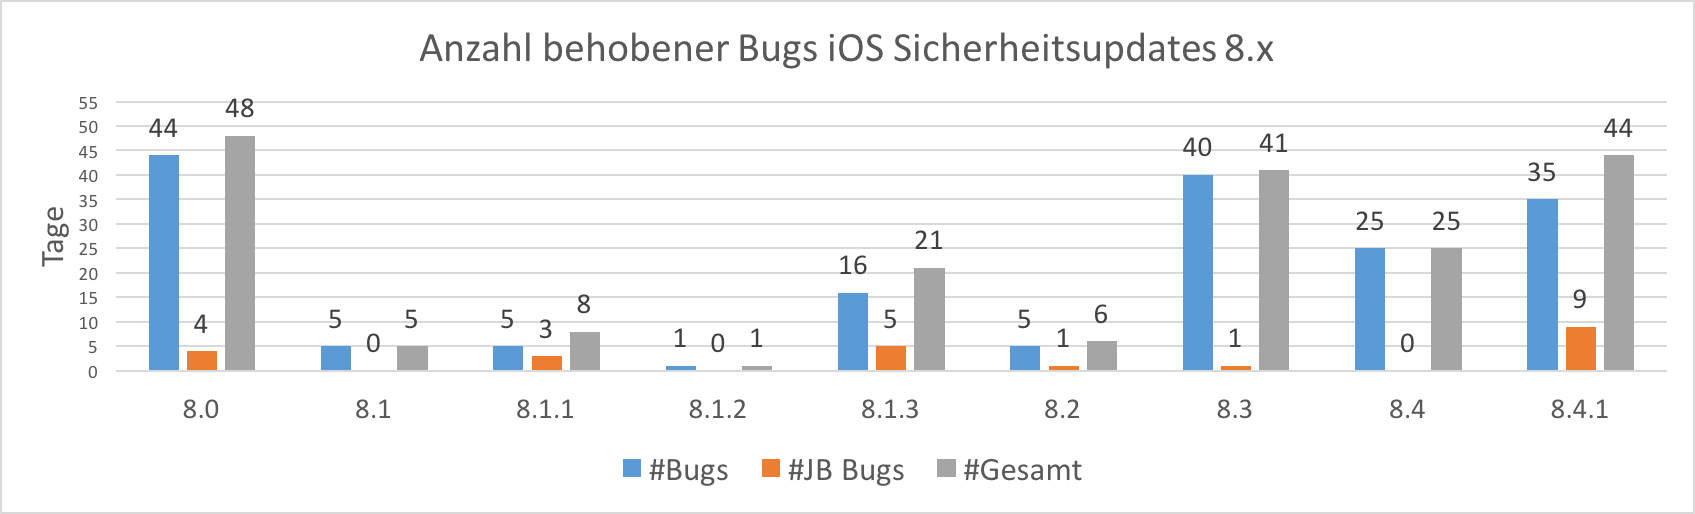
\includegraphics[scale=0.6]{Bilder/iOSSicherheitsupdate8.png}
        \caption{Anzahl Bugs iOS-Sicherheitsupdate iOS Version 8.x}
        \label{fig:AnalyseiOSSicherheitsupdate8}
\end{figure}

\begin{figure}[htbp]
        \centering
                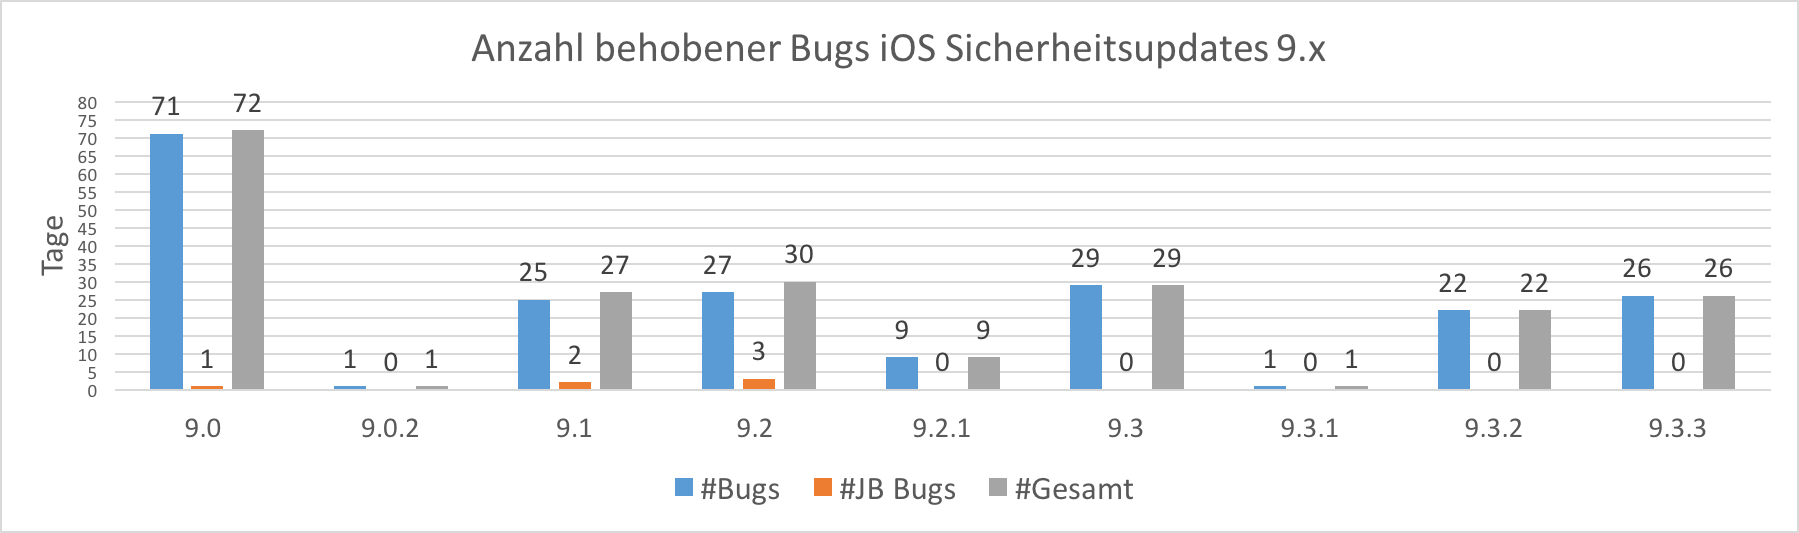
\includegraphics[scale=0.55]{Bilder/iOSSicherheitsupdate9.png}
        \caption{Anzahl Bugs iOS-Sicherheitsupdate iOS Version 9.x}
        \label{fig:AnalyseiOSSicherheitsupdate9}
\end{figure}


\newpage
\chapter{Tabellen}

